%! Author = bytelai
%! Date = 2021/11/11

% Preamble
\documentclass[UTF8]{ctexart}

% Packages
\usepackage{amsmath}
\usepackage{amsfonts}
\usepackage{textcomp}
\usepackage{graphicx}
\usepackage{url}
\usepackage{algorithm}
\usepackage{subfigure}
\usepackage{algorithmic}
\usepackage{bm}
\usepackage{natbib}
\newcommand{\myciteup}[1]{\textsuperscript{\textsuperscript{\cite{#1}}}}
%\usepackage[textwidth=14.5cm]{geometry}
%\usepackage{blindtext}
%\parindent=0pt
\title{基于TGV和灰度通道相似性的深度补全}
\author{lwj}
% Document
\begin{document}
    \begin{sloppypar}
    \maketitle
    \newpage
    \tableofcontents
    \newpage
    \section{利用优化实现颜色修复}
    \subsection{局部颜色相似性假设}
    深度恢复和颜色恢复从某种程度上是一样的,Levin\myciteup{levin2004}假设在邻域内,图像颜色存在线性相关性,他利用这种相关性对彩色图像进行了颜色恢复(colorization)的工作,Levin\myciteup{levin2004}提到相似性的两种度量方式如下:\\
    \begin{equation}
        w(i,j) \propto 1+\frac{1}{\sigma_{j}^{2}}(I(i) -\mu_i)(I(j)-\mu_i)
        \label{con:localSim1}
    \end{equation}
    \begin{equation}
        w(i,j) \propto \exp{\frac{-\left( I(i) - I(j) \right)^2}{2\sigma_{i}^2}}
        \label{con:localSim2}
    \end{equation}
    式\eqref{con:localSim1} 和 \eqref{con:localSim2}中 $w(i,j)$表示在$j$和$i$处颜色的线性因子,一个朴素的假设是不同通道局部相似性因子$w(i,j)$是相近的,因此在已知其中一个通道数据的情况下,其他通道的$w$,可以通过已知通道(例如灰度$I$)近似求解。\par
    \subsection{基于局部颜色相似性的颜色修复模型}
    对于$m$行$n$列的图像,假设已知某一通道的数据$I$,待恢复的颜色通道的数据为$f$,其中未知颜色数据的区域为$Z$,所有图像区域为$\Omega=[1,mn)$,$u,f\in R^{mn}$,$f(i) = 0,i \in Z $,通过求解损失函数\eqref{con:colorFidelity}最小值得问题 ,即可恢复缺失的颜色数据\par
    \begin{equation}
        J(u) = \sum\limits_{i\in Z} \left\| u(i) - \sum\limits_{j\in N(i,r),j\neq i}w(i,j)u(j) \right\|^2
        \label{con:colorFidelity}
    \end{equation}
    \eqref{con:colorFidelity}可以写成矩阵的形式:
    \begin{equation}
        \begin{aligned}
            J(u) &= \left\| \left( I - W \right) u - f \right\|^2\\
                 &= \sum\limits_{i\in Z}\left(  u(i)-\sum\limits_{j\in N(i,r)}w(i,j)u(j)\right)^2 + \sum\limits_{i\in \Omega\setminus Z}(u(i) - f(i))^2
            \label{con:JuMtx}
        \end{aligned}
    \end{equation}
    其中稀疏矩阵$W\in R^{mn\times mn}$如下
    \begin{equation}
        W(i,j) = \left\{
        \begin{array}{cc}
            \frac{w(i,j)}{\sum\limits_{j\in N(i,r),j\neq i}w(i,j)}&,j \in N(i,j),j \neq i, i\in Z\\
           0&, others\\
        \end{array} \right.
        \label{con:W}
    \end{equation}
    最小化\eqref{con:JuMtx}可以通过最小二乘法进行求解
    \begin{equation}
        u = \left( (I-W)^T(I-M) \right)^{-1}\left( I-W \right)^Tf
        \label{con:lsJu}
    \end{equation}\par
    \eqref{con:lsJu}可以通过$eigen$求解,但是实际发现求解稀疏矩阵线性问题的效率上,$matlab$会更高一些。\par
    \subsection{模型改进}
    此外flyfj\myciteup{flyfj2015}对\eqref{con:JuMtx}的一种改进为
    \begin{equation}
        \begin{aligned}
            J(u) &= \left\| \left( (\alpha_c G + I - W' \right) u - \alpha_c f \right\|^2, \alpha_c \in \left[ 0,1 \right]\\
                 &= \overbrace{\sum\limits_{i\in \Omega}\left(  u(i)-\sum\limits_{j\in N(i,r)}w(i,j)u(j)\right)^2}^{\mbox{约束项}} + \underbrace{\alpha_c\sum\limits_{i\in \Omega\setminus Z}(u(i) - f(i))^2}_{\mbox{保真项}}
        \end{aligned}
        \label{con:JuMtxAdvanced}
    \end{equation}\\
    \begin{equation}
        W'(i,j) = \left\{
        \begin{array}{cc}
            \frac{w(i,j)}{\sum\limits_{j\in N(i,r),j\neq i}w(i,j)}&,j \in N(i,j),j \neq i, i\in \Omega \\
            0&, others\\
        \end{array} \right.
        \label{con:WAdvanced}
    \end{equation}\\
    \begin{equation}
        G(i,j) = \left\{
        \begin{aligned}
            1&,i=j\ and\ f(i) \neq 0\\
            0&,others.
        \end{aligned}
        \right.
    \end{equation}
    相似性约束的范围也从未知图像区域$Z$扩展到整个图像区域$\Omega$,改进之后的模型能够更好的约束修复数据,不仅包含已知$\Omega\setminus Z$对$Z$的约束,同时$Z$对其他区域$\Omega\setminus Z$也被考虑进去了。引入了惩罚因子$\alpha_c$,表征保真项的权值。改进之后,其深度恢复效果得到很大的提升。图\ref{fig:colorize:onlyz}是仅使用未知区域约束项的效果,图\ref{fig:colorize:allregion}是使用全局约束项的效果,对应的惩罚因子$\alpha_c = 1.0$。可以看出深度修复的效果得到明显提升,一个原因是用来恢复深度信息的数据更多了。 \par
    \begin{figure}[htbp]
        \begin{minipage}[t]{0.5\linewidth}
            \centering
            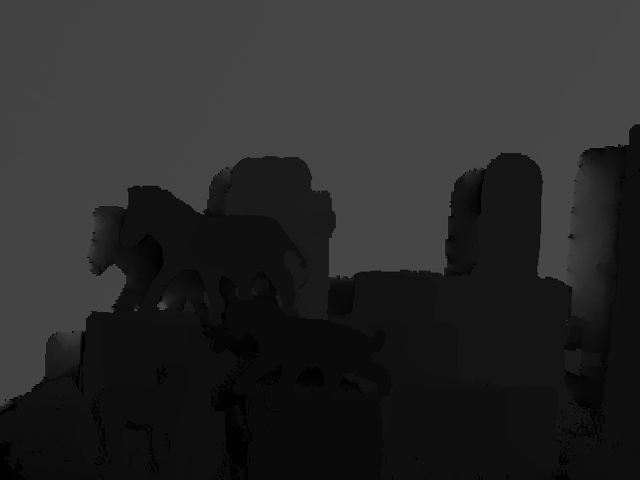
\includegraphics[scale=0.25]{figure/colorize_only_in_z.png}
            \caption{\small 只使用未知区域局部约束}
            \label{fig:colorize:onlyz}
        \end{minipage}
        \begin{minipage}[t]{0.5\linewidth}
            \centering
            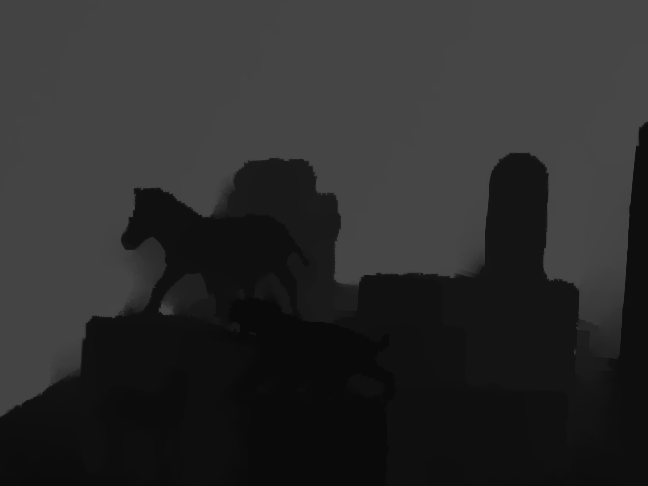
\includegraphics[scale=0.25]{figure/result_colorized_allregion_noseg.png}
            \caption{\small 使用了全局约束项}
            \label{fig:colorize:allregion}
        \end{minipage}
    \end{figure}\par
    另一种改进是针对线性系数$w(i,j)$的一种改进。Levin\myciteup{levin2004}的模型在图像边缘处的效果比较差,特别是未知区域$Z$和已知区域$Y=\Omega \setminus Z$的边缘正好和$rgb$图像边缘正好重叠的区域(见图\ref{fig:colorize:badregion}),由于该区域其他方向的深度信息不可用,而已知区域的深度信息对该区域又通过一个比较小的权值$w(i,j)$进行影响。这种区域在进行深度数据坐标系变换之后是非常常见的区域。
    \begin{figure}[htbp]
        \centering
        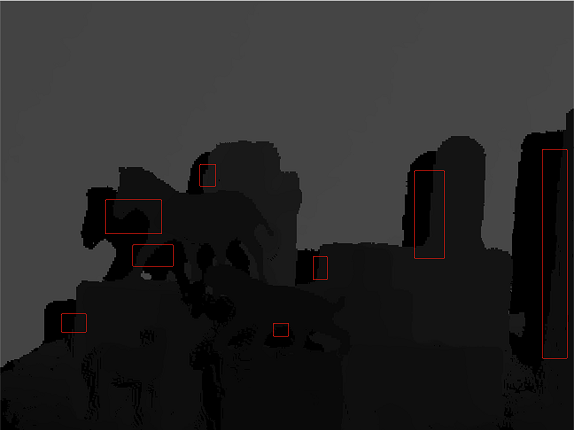
\includegraphics[scale=0.4]{figure/badRegion.png}
        \caption{\small 优化效果比较差的区域,图中红框}
        \label{fig:colorize:badregion}
    \end{figure}
    因此可以对图像进行语义分割,划分成不同的区块,对属于不同区块的权值$w(i,j)$直接置零。
    \begin{equation}
        W''(i,j) = \left\{
        \begin{array}{cc}
            \frac{w(i,j)}{\sum\limits_{j\in N(i,r),j\neq i}w(i,j)}&,j \neq i,seg(i)=seg(j),j \in N(i,j), i\in \Omega  \\
            0&, others\\
        \end{array} \right.
        \label{con:Wseg}
    \end{equation}\\
    其中$seg(i)$返回$i$处的所属的语义分割集合的$id$。如图由于减少了不同区域的错误影响,其优化效果得到一定的提升。
    \begin{figure}[htbp]
        \begin{minipage}[t]{0.5\linewidth}
            \centering
            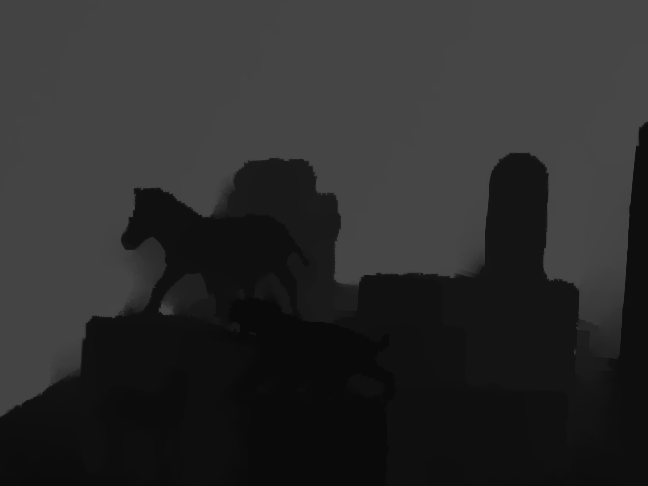
\includegraphics[scale=0.25]{figure/result_colorized_allregion_noseg.png}
            \caption{\small 使用全局约束但是没有利用语义分割}
            \label{fig:colorize:noseg}
        \end{minipage}
        \begin{minipage}[t]{0.5\linewidth}
            \centering
            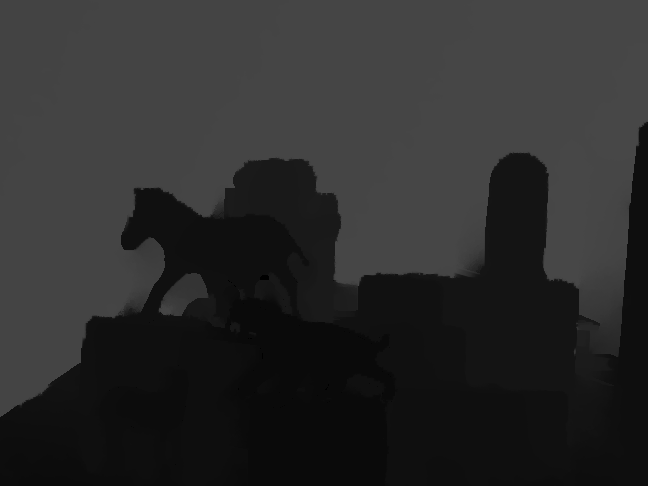
\includegraphics[scale=0.25]{figure/result_colorized_allregion_seg.png}
            \caption{\small 利用语义分割优化全局约束}
            \label{fig:colorize:seg}
        \end{minipage}
    \end{figure}\par
    由于将属于不同区域的权值置零了。矩阵$W'$的稀疏程度增加,容易产生奇异性。需要进一步考虑算法处理。\par


\section{基于tgv的深度数据恢复}
    \subsection{ITGV}
    Ranftl\myciteup{Ranftl2012}提出使用Nagel-Enkelmann算子\myciteup{Nagel1986}将结构信息融入到TGV模型中的正则化手段ITGV。其公式如\eqref{con:itgv}
    \begin{equation}
        ITGV^{2}_{\alpha}(u) = \min\limits_{w \in \mathbb{R}^2}\left\{ \alpha_u \int_{\Omega}\left|D^\frac{1}{2} \nabla u - w \right|dx + \alpha_w\int_{\Omega}\left|\nabla w\right|dx \right\}
        \label{con:itgv}
    \end{equation}
    其中的$D^{\frac{1}{2}}$为Nagel-Enkelmann算子
    \begin{equation}
        D^{\frac{1}{2}} = \exp{\left(-\gamma \left| \nabla I_L  \right|^{\beta}  \right)}nn^T+n^\perp{n^\perp}^T
        \label{con:nagel-EnkelmannOp}
    \end{equation}
    $n$是图像梯度的方向,$n=\frac{\nabla I_L}{\left| \nabla I_L \right|}$,$n^\perp$垂直于$n$,$\gamma$和$\beta$是自定义参数。
    Ferstl\myciteup{Ferstl2013}进一步的提出,用ITGV进行深度数据上采样的方法,并取得了较好的效果。其模型见下式\eqref{con:Itgv4DepthUpsample}
    \begin{equation}
        J(u,w) = ITGV^2_{\alpha}(u,w) + \int_{\Omega}\lambda\left| u-f \right|^2 dx
        \label{con:Itgv4DepthUpsample}
    \end{equation}
    其中系数$\lambda$在深度数据缺失的区域为零。即$\lambda(i) = 0, i\in Z$。TGV正则化,能够在保留边缘的同时,去除噪声,在已有深度数据的区域$D=\Omega\setminus Z$ 由于其具有各项异性的传播特性,能够衰减梯度方向的传播,保留梯度切线方向的传播,因此能够比较好的保留原始图像的边缘信息,但是在深度为零的区域,这种正则化作用由于没有原始数据的边缘梯度做为参考,这种正则化作用就被减弱了。因此通过引入结构化参数$D^{\frac{1}{2}}$将灰度通道的数据的边缘信息作为参照,保证了ITGV在深度缺失区域的各项异性。\par

\subsection{STGV}
    Drozdov进一步的提出改进的边缘算子\myciteup{Drozdov2016}用于深度恢复。并在已有的数据集上取得了不错的效果。STGV基于超像素技术,将rgb图像进行超像素处理,计算每个超像素内的深度分布,提出异常点,利用$DBSCAN$聚类算法实现超像素的合并。同时利用贪婪算法,保证每个超像素块内的已知深度区域具有足够的比例。利用超像素信息,进一步加强边缘算子的各向异性,见式\eqref{con:Dadvanced}。
    \begin{equation}
        \mathbb{D} = \Gamma nn^T + n^{\perp}{n^{\perp}}^{T}
        \label{con:Dadvanced}
    \end{equation}
    其中$\Gamma$为边缘指示函数,见式\eqref{con:edge},
    \begin{equation}
       \Gamma = \left\{
       \begin{aligned}
           1 \ & inside\ segment,\\
           0 \ & segment\ border
       \end{aligned}
       \right.
        \label{con:edge}
    \end{equation}
    将式\eqref{con:Dadvanced}代入式\eqref{con:Itgv4DepthUpsample}中得到
    \begin{equation}
        J(u) = \min\limits_{w \in \mathbb{R}^2}\left\{ \alpha_u \int_{\Omega}\left|\mathbb(D) \nabla u - w \right|dx + \alpha_w\int_{\Omega}\left|\nabla w\right|dx \right\} + \int_{\Omega\setminus Z}\lambda\left| u-f \right|^2 dx
        \label{con:stgvLossFun}
    \end{equation}
    超像素边缘在一定程度是贴合物体的轮廓,在超像素边缘(一定程度上也是图像边缘)区域,通过\eqref{con:edge}完全抑制了法线方向的扩散,深度修复具有各向异性。而在超像素内部,具有各向同性传播。因此STGV能够取得由于ITGV的效果。见图\ref{fig:itgv}和\ref{fig:stgv},迭代了14730次(耗时1009秒),参数为:$\alpha_w=5,\alpha_u=1.2,\lambda=50,\gamma=0.85,\beta=9$。
    \begin{figure}[htbp]
        \begin{minipage}[t]{0.5\linewidth}
            \centering
            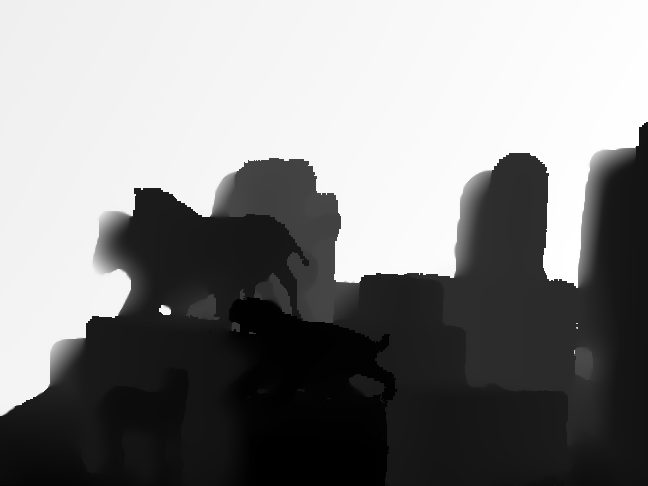
\includegraphics[width=0.9\linewidth]{figure/tgvl2_14730_1009s_noseg}
            \caption{ITGV深度修复效果}
            \label{fig:itgv}
        \end{minipage}
        \begin{minipage}[t]{0.5\linewidth}
            \centering
            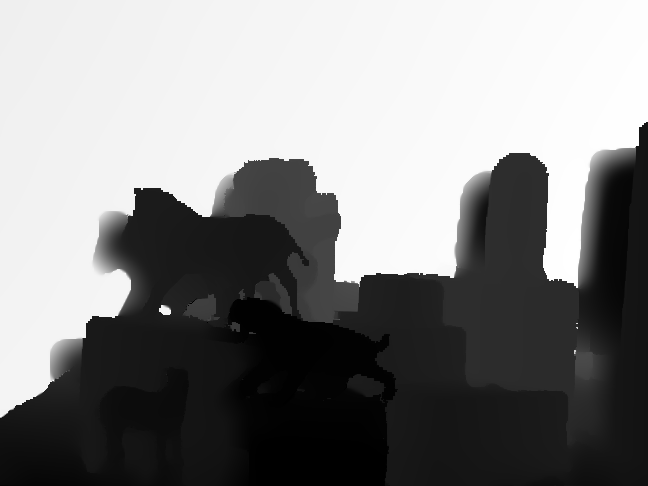
\includegraphics[width=0.9\linewidth]{figure/tgvl2_14730_user_seg}
            \caption{STGV效果(图像边缘经过手动调整)}
            \label{fig:stgv}
        \end{minipage}
    \end{figure}\par

    STGV存在一下几个问题:
    \begin{itemize}
        \item [1)]
        效果严重依赖超像素算法对边缘识别的准确度,如果边缘识别错误,则深度修复会带来很严重的错误,修复效果还不如ITGV正则化的效果,见图\ref{fig:wrongSuperPix}和图\ref{fig:wrongspDepInpaint}
        \item [2)]
        优化算法需要迭代很久才能够收敛。对于$648\times486$分辨率的数据,在$I7\ GTX2080$配置的电脑上跑了数个小时都优化不出来。
    \end{itemize}
    \begin{figure}[htbp]
        \begin{minipage}[t]{0.5\linewidth}
            \centering
            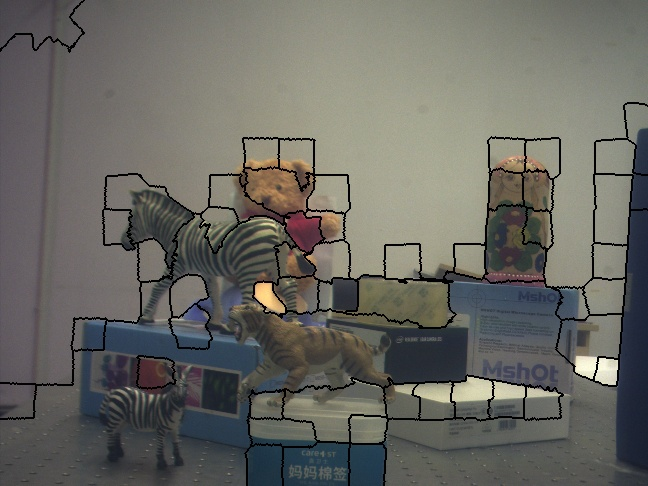
\includegraphics[width=0.9\linewidth]{figure/wrongseg}
            \caption{\small 错误的超像素结果}
            \label{fig:wrongSuperPix}
        \end{minipage}
        \begin{minipage}[t]{0.5\linewidth}
            \centering
            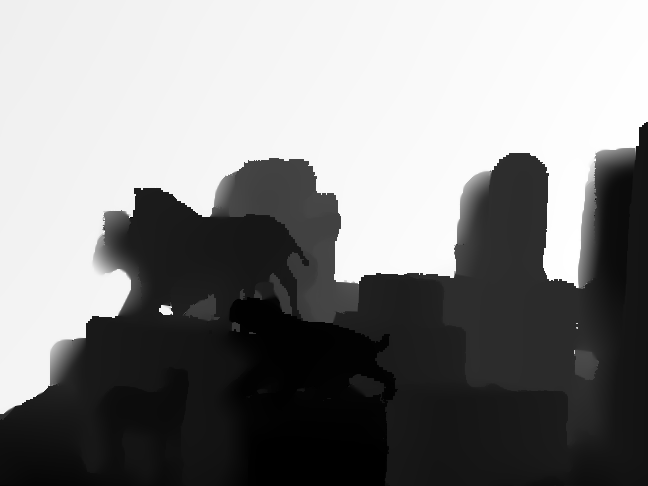
\includegraphics[width=0.9\linewidth]{figure/iter14740_wrongseg}
            \caption{\small 错误超像素产生的深度修复效果}
            \label{fig:wrongspDepInpaint}
        \end{minipage}
    \end{figure}
    \emph{注意,为了增加图像对比度,图\ref{fig:itgv},\ref{fig:stgv},\ref{fig:wrongspDepInpaint}做了最大值归一化处理。后续深度图如无特殊说明,均做了同样的处理}
\subsection{TGV收敛问题}
    TGV问题一般使用交替方向乘子法($Alternating\ Direction\ Method\ of\
    Multipliers, ADMM$求解。Chambolle\myciteup{Chambolle2011}提出了基于prime-dual的算法实现,见算法\ref{alg:pdAlg1},收敛速度优于交替方向乘子法。
    对于求解鞍点问题\eqref{con:pd-init}
    \begin{equation}
        \min\limits_{x\in X} \max \limits_{y \in Y} \left< Kx,y \right> + G(x) - F^*(y)
        \label{con:pd-init}
    \end{equation}
    其中$\left< \cdot,\cdot \right>$ 表示对偶积,离散情况下可以看成是向量的点乘。可以使用算法\ref{alg:pdAlg1}进行求解。
    \begin{algorithm}
        \caption{pdAlg1}
        \begin{algorithmic}
            \STATE Initialization: $Choose \tau ,\sigma > 0,\theta \in [0,1],(x^0,y^0)\in X\times Y \ and \ set\ \overline{x}^0=x^0. s.t. \tau \sigma L^2<1$
            \STATE Iterations($n\geq 0$):\ $Update\ x^n,y^n,\overline{x}^n\ as\ follows:$
            \begin{equation}
                \left\{
                \begin{aligned}
                    y^{n+1} &= (I+\sigma \partial F^*)^{-1}(y^n+\sigma K\overline{x}^n)\\
                    x^{n+1} &= (I+\tau \partial G)^{-1}(x^n-\tau K^* y^{n+1})\\
                    \overline{x}^{n+1} &=x^{n+1} + \theta (x^{n+1}-x^n)
                \end{aligned}
                \right.
            \end{equation}
        \end{algorithmic}
        \label{alg:pdAlg1}
    \end{algorithm}
    其中$L=\left\| K \right\|$表示算子$K$的范数。\par

    针对$K$比较复杂的情况,其范数往往比较难计算,可以根据Pock\myciteup{Diagonal_preconditioning}提到的做法,用算法\ref{alg:pdPrecondition}求解
    \begin{algorithm}
        \caption{pdPrecondition}
        \begin{algorithmic}
            \STATE $\bm{Initialization}$: $Choose \tau_0,\sigma_0 >0\ with\ \tau_0\sigma_{0}L^2\leq 1, (x^0,y^0)\in X\times Y \ and \ set\ \overline{x}^0=x^0.$
            \STATE $\bm{Caculate\ Tensors}$:$Choose\ \alpha \in[0,2]\ and\ Caculate\ as\ follow:$
            \begin{equation}
                \begin{aligned}
            T &= diag(\bm{\tau}) , where\ \bm{\tau} = (\tau_1,...,\tau_n),\tau_j=\frac{1}{\sum_{i=1}^m\left| K_{i,j} \right|^{2-\alpha}},\\
            \Sigma &= diag(\bm{\sigma}),where\ \bm{\sigma} = (\sigma_1,...,\sigma_m).\sigma_i=\frac{1}{\sum_{j=1}^n\left| K_{i,j} \right|^{\alpha}}\\
                \end{aligned}
            \end{equation}
        \STATE $\bm{Iterations}(k\geq 0)$:\ $Update\ x^n,y^n,\overline{x}^n\ as\ follows:$
            \begin{equation}
                \begin{aligned}
                    x^{k+1} &=(I+\tau_k T\partial G)^{-1}(x^k-\tau_k TK^Ty^k ), \\
                    y^{k+1} &=(I+\sigma_k\Sigma\partial F^*)(y^k+\sigma_k \Sigma K\overline{x}^k).\\
                    \theta_k &= \frac{1}{\sqrt {1+2\gamma \tau_k}},\tau_{k+1}=\theta_k\tau_k,\sigma_{k+1}=\frac{\sigma_k}{\tau_n}\\
                    \overline{x}^{k+1} &= x^{k+1}+\theta_k(x^{k+1}-x^k)\\
                \end{aligned}
            \end{equation}
        \end{algorithmic}
        \label{alg:pdPrecondition}
    \end{algorithm}
    算法\ref{alg:pdPrecondition}可以看成是Chambolle\myciteup{Chambolle2011}提到的$Algorithm 2.$和Pock\myciteup{Diagonal_preconditioning}提到的算法的结合版本。\par
\section{TGV和colorize结合}
    可以考虑将TGV和colorize结合,优化图像效果。具体做了两种尝试:\par
    \subsection{利用COLORIZE作为保真项}
    一种思路是将\eqref{con:JuMtxAdvanced}\eqref{con:WAdvanced}作为保真项,采用TGV作为正则化,进行问题的求解,如式\eqref{con:cstgv}。下面简称为CSTGV(colorized superpixel total generize variation)。
    \begin{equation}
        J(u,w) = \alpha_u \sum \left|\mathbb{D}(\nabla u-w) \right| + \alpha_w \sum \left| \xi w \right| + \sum \frac{1}{2\lambda} \left\|   Au-\alpha_c f \right\|^2
        \label{con:cstgv}
    \end{equation}
    其中$A=\alpha_{c}G+I-W'$,通过灰度数据可以计算出来。$Au$可以通过matlab实现。
    采用改进的prime-dual算法来实现优化,原始的问题\eqref{con:cstgv}的$Fenchel-Legendre$对偶形式为:
    \begin{equation}
        \begin{aligned}
            \mathop {\min}\limits_{(u,w)\in U\times V} \max \limits_{(p,q,r)\in V \times W \times U}
            \overbrace{\left< \mathbb{D}(\nabla u-w),p\right> + \left< \xi w,q \right> + \left< W'u,r \right>}^{\left< Kx,y \right>}\\
            -\underbrace{ \left[ \left< \alpha_c f,r \right> + \frac{\lambda}{2}\left\| r \right\|^2
            + \mathbb{I}_{\left\{\left\|\cdot\right\|_\infty \leq \alpha_u\right\}}(p)
                + \mathbb{I}_{\left\{\left\|\cdot\right\|_\infty \leq \alpha_w\right\}}(q)\right]
            }_{F^*(y)}
        \end{aligned}
        \label{con:pd-Ju}
    \end{equation}
    对应于式\eqref{con:pd-init}式\eqref{con:pd-Ju}中的$G(x)=0$,$K$如下
    \begin{equation}
        K=\begin{bmatrix}
              \mathbb{D} \nabla \ & -\mathbb{D}\\
              0                        & \xi \\
              A                      &   0
        \end{bmatrix}
        \label{con:K}
    \end{equation}
    其中的差分算子$\nabla$使用前向差分算子,对$m$行$n$列的图像
    \begin{equation}
        \begin{aligned}
        \nabla &= \begin{bmatrix}
                     \nabla_x\\
                     \nabla_y
        \end{bmatrix}\\
            \nabla_x &= I_m \otimes \nabla_f\\
            \nabla_y &= \nabla_f \otimes I_m
        \end{aligned}
    \end{equation}
    其中$\otimes$表示Kronecker内积。$I_m$是$m\times m$维的单位矩阵,$\nabla_f$表示带有循环边界的一维差分算子,$\nabla_f\in R^{n\times n}$。
    \begin{equation}
        \nabla_f=\begin{bmatrix}
                     -1 &1      &0      &0\\
                     0  &\ddots &\ddots &0\\
                     0  &0      &-1     &1\\
                     1  &0      &0      &-1
        \end{bmatrix}
    \end{equation}
    \begin{figure}[htbp]
        \begin{minipage}[t]{0.5\linewidth}
            \centering
            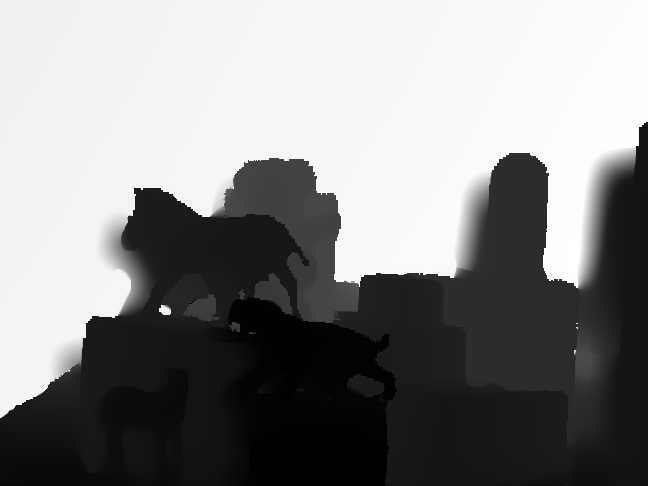
\includegraphics[width=0.9\linewidth]{figure/stgvl2_54740iter_4562s}
            \caption{\small STGV原始效果}
            \label{fig:stgv_54740}
        \end{minipage}
        \begin{minipage}[t]{0.5\linewidth}
            \centering
            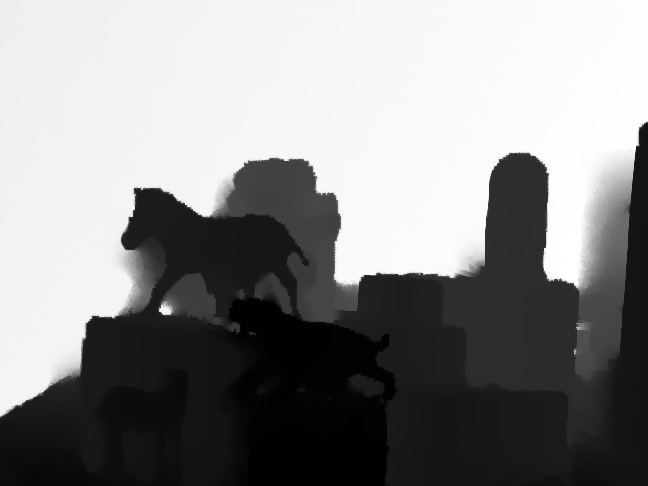
\includegraphics[width=0.8\linewidth]{figure/stgvColorF_54740iter_4562s}
            \caption{\small colorize保真项CSTGV优化效果}
            \label{fig:cstgv_54740}
        \end{minipage}
    \end{figure}
    图\ref{fig:stgv_54740}和图\ref{fig:cstgv_54740}分别是$STGV$和$CSTGV$的优化效果。用到的参数为:$itertimes=54740,\alpha_w=5,\alpha_u=1.2\lambda=1e-2$(式\eqref{con:cstgv}的$\lambda$和\eqref{con:Itgv4DepthUpsample}的$\lambda$不同)。对于图像恢复,调节保真项权值$\lambda$能够提升效果。如图\ref{fig:cstgv_1e-4}和\ref{fig:stgv_1e-4},在$itertimes=54740,\alpha_w=5,\alpha_u=1.2,\lambda=1e-4$参数下,效果明显优于图\ref{fig:stgv_54740}和图\ref{fig:cstgv_54740}
    \begin{figure}[htbp]
        \begin{minipage}[t]{0.5\linewidth}
            \centering
            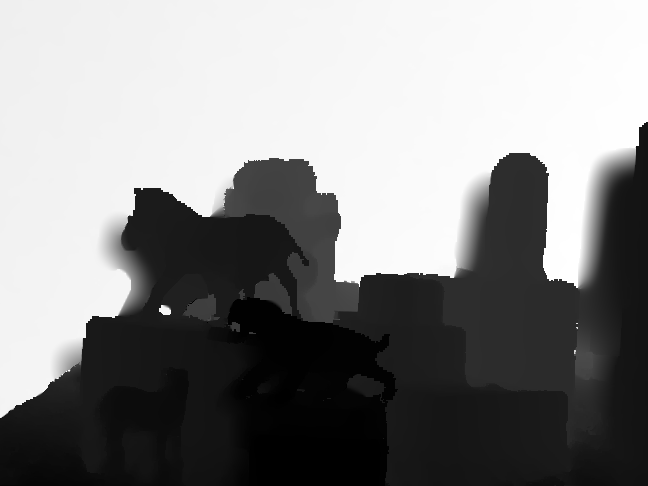
\includegraphics[width=0.9\linewidth]{figure/tgvl2_iter54740_lambda1e-4}
            \caption{\small STGV \ $ \lambda=1e-4,$耗时4051.26s}
            \label{fig:stgv_1e-4}
        \end{minipage}
        \begin{minipage}[t]{0.5\linewidth}
            \centering
            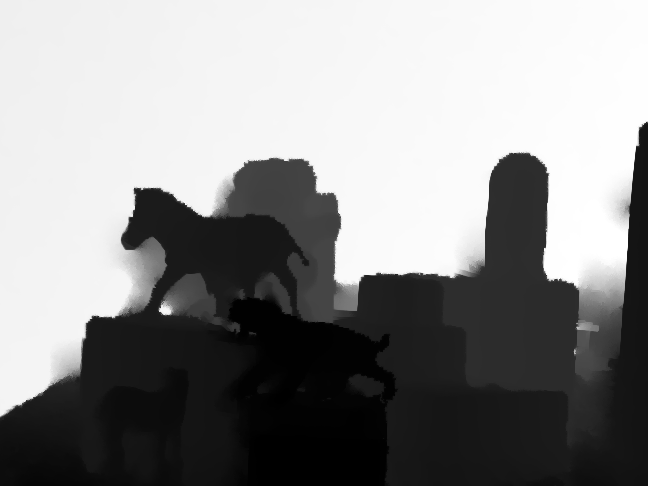
\includegraphics[width=0.9\linewidth]{figure/tgvColorF_iter54740_lamda1e-4}
            \caption{\small CSTGV\ $\lambda=1e-4,$耗时5253s}
            \label{fig:cstgv_1e-4}
        \end{minipage}
    \end{figure}\par
\subsection{利用COLORIZE优化后的结果作为初始值进行STGV优化}
    STGV收敛速度慢的一个解决手段,可以通过选取合适的初始值来解决。而colorize得到的结果存在比较多的毛刺,可以简单的将两个算法流程串联。以提升效果。需要注意的是,colorize得到的结果(记为$g$)和原始输入$f$需要经过相同的归一化因子归一化,否则会导致尺度上的错误。效果见图\ref{fig:colorize_tgv}\par
    \begin{figure}[htbp]
        \centering
        \subfigure[colorize no using seg]{
            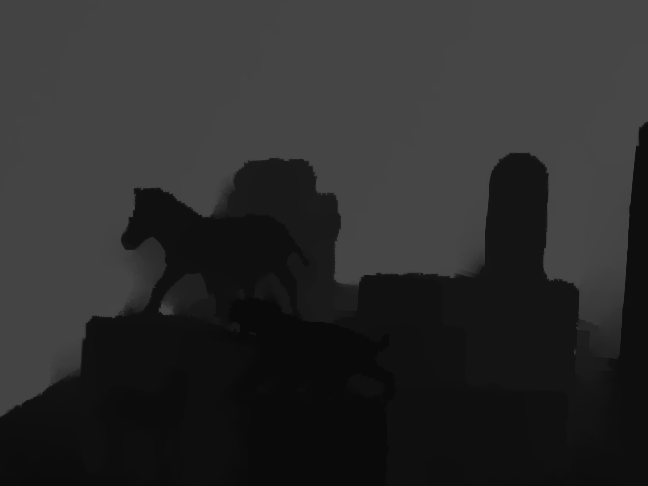
\includegraphics[width=0.45\linewidth]{figure/result_colorized_allregion_noseg}
%            \caption{\small 直接使用\eqref{fig:colorize:noseg}}
        }
        \quad
        \subfigure[colorize using seg]{
        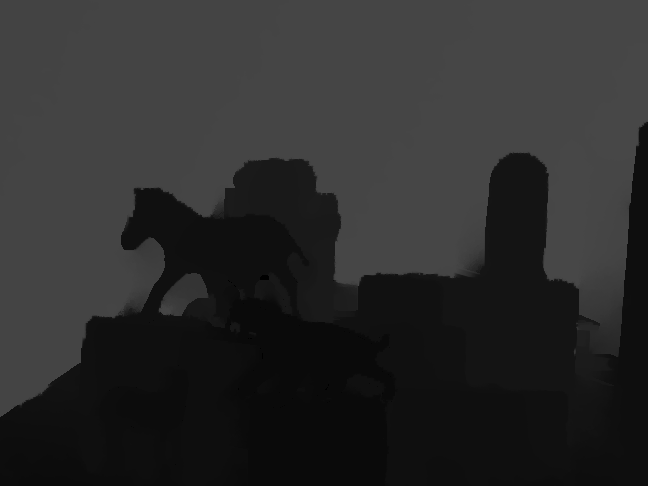
\includegraphics[width=0.45\linewidth]{figure/result_colorized_allregion_seg}
        }
        \quad
        \subfigure[colorize no seg then stgv]{
        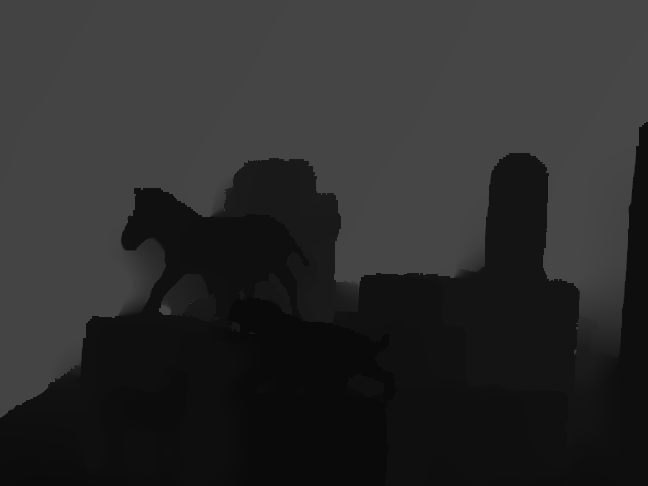
\includegraphics[width=0.45\linewidth]{figure/result_colorized_tgv}
        }
        \quad
        \subfigure[colorize using seg then stgv]{
        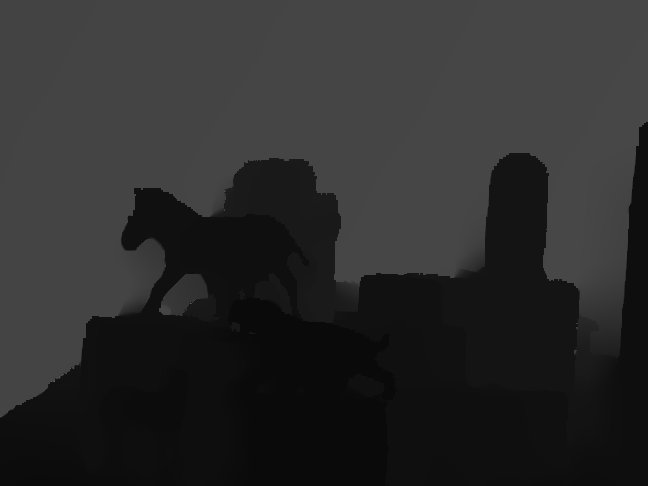
\includegraphics[width=0.45\linewidth]{figure/result_colorizedseg_tgv}
        }
        \caption{\small 对colorize优化后的图像进行tgv平滑操作}
        \label{fig:colorize_tgv}
    \end{figure}
    使用参数为$\alpha_u = 1.2,\alpha_w=4.5,\lambda=40,itertimes=2000$
    \subsection{接下来的工作}
    研究其他的深度修复算法,同时考虑完善现有算法的一些细节,
    \begin{itemize}
        \item 使用分割信息之后colorize的奇异问题;
        \item tgv收敛和算法\ref{alg:pdPrecondition}中参数$\gamma$的关系
        \item c++实现和matlab实现的colorize算法存在局部数据差异
        \item matlab实现cstgv,并测试效果
        \item 完善原先代码前向循环边界差分部分
    \end{itemize}




%\begin{equation}
%    s.t \theta \in [0,1],(x^0,y^0)\in X \times Y
%\end{equation}



\bibliography{references}
    \bibliographystyle{unsrt}

    \end{sloppypar}
\end{document}
